\documentclass[]{article}
%\documentclass[11pt, oneside]{article}          % use "amsart" instead of "article" for AMSLaTeX format
\usepackage{geometry}                           % See geometry.pdf to learn the layout options. There are lots.
\geometry{letterpaper}                                  % ... or a4paper or a5paper or ... 
%\geometry{landscape}                           % Activate for rotated page geometry
%\usepackage[parfill]{parskip}                  % Activate to begin paragraphs with an empty line rather than an indent
\usepackage{graphicx}                           % Use pdf, png, jpg, or eps§ with pdflatex; use eps in DVI mode
                                                                % TeX will automatically convert eps --> pdf in pdflatex                
\usepackage{amssymb}
\usepackage{upquote}

%-----------------------------------------------------------------------------
% Special-purpose color definitions (dark enough to print OK in black and white)
\usepackage{color}
% A few colors to replace the defaults for certain link types
\definecolor{orange}{cmyk}{0,0.4,0.8,0.2}
\definecolor{darkorange}{rgb}{.71,0.21,0.01}
\definecolor{darkgreen}{rgb}{.12,.54,.11}
%-----------------------------------------------------------------------------
% The hyperref package gives us a pdf with properly built
% internal navigation ('pdf bookmarks' for the table of contents,
% internal cross-reference links, web links for URLs, etc.)
\usepackage{hyperref}
\hypersetup{pdftex, % needed for pdflatex
  breaklinks=true, % so long urls are correctly broken across lines
  colorlinks=true,
  urlcolor=blue,
  linkcolor=darkorange,
  citecolor=darkgreen,
}


\date{}

\begin{document}

\title{Reproducible Applied Statistics:\\
Is tagging of therapist-patient interactions reliable?\thanks{Submitted
to \url{https://github.com/BIDS/repro-case-studies}.
}}

\author{K. Jarrod Millman (JM)\\ Division of Biostatistics\\ UC Berkeley \and
Kellie Ottoboni (KO)\\ Department of Statistics\\ UC Berkeley \and
Naomi A. P. Stark (NS)\\ Department of Philosophy\\ University of Pennsylvania \and
Philip B. Stark (PS)\\ Department of Statistics\\ UC Berkeley
}


\maketitle


\section{Introduction}

This case study illustrates some of the reproducible practices we (JM, KO, PS)
have adopted when working with scientific or domain experts as applied
statisticians.

\begin{enumerate}
\def\labelenumi{\arabic{enumi})}
\itemsep1pt\parskip0pt\parsep0pt
\item
  Who are you and what is your research field?
\end{enumerate}

%\begin{itemize}
%\itemsep1pt\parskip0pt\parsep0pt
%\item
%  K. Jarrod Millman, Division of Biostatistics, UC Berkeley PhD student
%  in biostatistics; background in scientific computing and neuroscience
%\item
%  Kellie Ottoboni, Department of Statistics, UC Berkeley PhD student in
%  statistics
%\item
%  Naomi A.P. Stark, Department of Philosophy, University of Pennsylvania
%  Undergraduate in bioethics; background in therapy with children on the
%  autistic spectrum
%\item
%  Philip B. Stark, Department of Statistics, UC Berkeley Faculty in
%  statistics; background in physical science
%\end{itemize}

We are three applied statisticians~(JM,~KO,~PS) at Berkeley working with a
domain specialist~(NP) at the University of Pennsylvania. Our case study
involves assessing inter-rater reliability (IRR) for human classifiers of
therapy sessions with children on the autistic spectrum.

\begin{enumerate}
\def\labelenumi{\arabic{enumi})}
\setcounter{enumi}{1}
\itemsep1pt\parskip0pt\parsep0pt
\item
  Define what the term ``reproducibility'' means to you generally and/or
  in the particular context of your case study.
\end{enumerate}

The term \emph{reproducibility} is overloaded with orthogonal or even
contradictory meanings in different disciplines. In the context of the current
project, \emph{reproducibility} means that we have documented (nearly) every
step of the analysis, from cleaning to coding to code execution. Of course, the
project itself is \emph{about} the \emph{reliability and replicability} of a
particular kind of measurement: raters' assessments of activities during
therapy sessions.

\newpage

\section{Workflow diagram}\label{workflow-diagram}

%\begin{figure}[h]
%  \centering
%    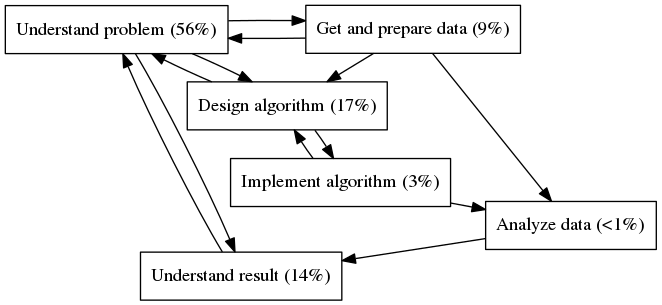
\includegraphics[width=0.5\textwidth]{work_process.png}
%  \caption{The nodes represent the following stages of our investigation
%           (1) understanding the fundamental problem, (2) data acquisition,
%           pre-processing, and cleaning, (3) algorithm design and analysis,
%           (4) code development, (5) data analysis, and (6) reflection and
%           synthesis.}
%\end{figure}

\begin{figure}[h]
  \centering
    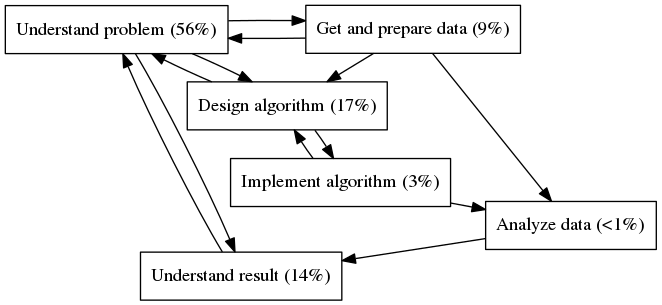
\includegraphics[width=0.5\textwidth]{work_process.png}
  \caption{Each box corresponds to one aspect involved in a typical applied
           statistic project.  The edges represent influence.  For instance,
           the arrow pointing from the box labeled \texttt{Understand problem}
           to \texttt{Acquire data} represents the fact that our understanding
           of the problem influenced how we acquired the data.  We will describe
           the work corresponding to labeled box in more detail in our
           workflow narrative below.  In any specific applied statistics project,
           the amount of time we spend on each aspect varies as does the
           way each aspect of the project influences our work on other
           aspects.}
\end{figure}

\section{Workflow narrative}\label{workflow-narrative}

%Referring to your diagram, describe your workflow for this specific
%project, from soup to nuts. Imagine walking a friend or a colleague
%through the basic steps, paying particular attention to links between
%steps. Don't forget to include ``messy parts'', loops, aborted efforts,
%and failures.
%
%It may be helpful to consider the following questions, where
%interesting, applicable, and non-obvious from context. For each part of
%your workflow:
%
%\begin{itemize}
%\itemsep1pt\parskip0pt\parsep0pt
%\item
%  \textbf{Frequency:} How often does the step happen and how long does
%  it take?
%\item
%  \textbf{Who:} Which members of your team participate (or not)?
%\item
%  \textbf{Manual/Automated:} Is the step automated or does it involve
%  human intervention (if so, is it recorded)?
%\item
%  \textbf{Tools:} Which software or online tools are used in the step?
%  How are they used?
%\end{itemize}
%
%In addition to detailing the steps of the workflow, you may wish to
%consider the following questions about the workflow as a whole:
%
%\begin{itemize}
%\itemsep1pt\parskip0pt\parsep0pt
%\item
%  \textbf{Data:} Is your raw data online? \textbf{yes}
%\item
%  Is it citeable?
%\item
%  Does the license allow external researchers to publish a
%%  replication/confirmation of your published work? \textbf{yes}
%\item
%  \textbf{Software:} Is the software online? \textbf{yes}
%\item
%  Is there documentation? \textbf{yes}
%\item
%  Are there tests? \textbf{yes}
%\item
%  Are there example input files alongside the code? \textbf{yes}
%\item
%  \textbf{Processing:} Is your data processing workflow online?
%  \textbf{everything downstream of data anonymization}
%\item
%%  Are the scripts documented? \textbf{yes}
%\item
%  Would an external researcher know what order to run them in?
%  \textbf{yes}
%\item
%  Would they know what parameters to use? \textbf{yes}
%\end{itemize}
%
%\emph{(500-800 words)}

Following best practices in open source software development
\cite{millman2014developing}, we've created a Python package for permutation
tests and confidence sets called \texttt{permute}.
In this case study, we will illustrate how we leverage the software
infrastructure of \texttt{permute} to conduct reproducible and collaborative
applied statistics research with our scientific collaborators.


We cleaned the data, developed a nonparametric approach to assessing IRR
appropriate to the experiment, implemented the approach in Python,
incorporated the resulting code into an evolving Python package of
permutation tests (\texttt{permute}), applied the approach to the cleaned
data, documented the code and the analysis, and wrote up the results in
a LaTeX document. 

\subsection{Understanding the fundamental problem}

In this study, our scientific collaborators (domain experts?) were interested
in:  What happens in therapy session with autistic kids?
In particular, they wanted to know whether humans can reliably rate different
behaviors?
To this end, they designed an experiment to determine whether humans could
reliably assess different behaviors reliably.


  \begin{enumerate}
  \def\labelenumii{\roman{enumii}.}
  \itemsep1pt\parskip0pt\parsep0pt
  \item
    conversations between N. Stark and (primarily) P. Stark to
    understand the experimental set-up. Time: approximately 10 1-hour
    meetings
  \item
    met regularly (approximately weekly, sometimes more) as a team to
    discuss the project, work on whiteboards, and use pair programming
    (J. Millman, K. Ottoboni, P. Stark) Time: approximately 10 2-hour
    meetings.
  \end{enumerate}
  

\subsection{Data acquisition, pre-processing, and cleaning}

The data were collected by Naomi Stark and Gil Kliman. They
comprise ratings of segments of 8 videos by 10 trained raters. Each
video is divided into approximately 40 time segments. In each time
segment, none, any, or all of 183 types of activity might be taking
place. The raters indicated which of those activities was taking place
during each segment of each video.

  \begin{enumerate}
  \def\labelenumii{\roman{enumii}.}
  \itemsep1pt\parskip0pt\parsep0pt
  \item
    receipt of preliminary data as an Excel spreadsheet; understanding
    the ``data dictionary''; vetting for obvious errors (P. Stark) Time:
    approximately 1 hour
  \item
    several ``trips to the well'' before getting a version of the data
    that did not have obvious errors (P. Stark) Time: approximately 4
    hours
  \item
    export the Excel data to .csv format (P. Stark) Time: approximately
    5 minutes.
  \item
    data anonymization: substitute unique numerical identifiers for
    raters' names. This step was performed using regular expressions in
    an interactive text editor, on the .csv file. It was not performed
    reproducibly (i.e., not scripted), but it can be checked readily.
    (P. Stark) Time: approximately 1 hour.
  \item
    screen the anonymized data for transcription errors, typos, etc. (J.
    Millman, P. Stark) Time: approximately 5 hours
  \item
    develop sed scripts to ``correct'' the data for duplicated entries
    and inferred typos (J. Millman) Time: included above
  \item
    send cleaned data to N. Stark to verify that the corrections were
    appropriate (P. Stark, N. Stark) Time: 1 hour
  \item
    include cleaned data in git repo: the anonymized data are public,
    pre- and post-cleaning
  \end{enumerate}
  
\subsection{Algorithm development}

  \begin{enumerate}
  \def\labelenumii{\roman{enumii}.}
  \itemsep1pt\parskip0pt\parsep0pt
  \item
    ``Problem appreciation'': conversations culminating in the decision
    to assess the reliability one category at a time. (J. Millman, K.
    Ottoboni, P. Stark) Time: approximately 4h.
  \item
    Developed an understanding that it was best to treat the videos
    separately
  \item
    Searched the literature for extant approaches to assessing IRR. We
    determined that there was no suitable method, in part because the
    experiment was stratified and in part because standard methods make
    indefensible parametric assumptions, which we hoped to avoid (P.
    Stark) Time: 3h
  \item
    Decided to use permutation tests
  \item
    Decided what the appropriate permutation would be: permuting each
    rater's ratings within a video, independently across raters and
    across videos.
  \item
    Chose a test statistic to use within each stratum: concordance of
    ratings
  \item
    Derived a simple expression for computing the concordance
    efficiently (J. Millman, P. Stark) Time: 1h
  \item
    Decided how to combine tests across strata: nonparametric
    combination of tests, NPC (J. Millman, K. Ottoboni, P. Stark) Time:
    1h
  \item
    Developed a computationally efficient approach to finding the
    overall p-value for NPC (J. Millman, K. Ottoboni, P. Stark) Time:
    1.5h
  \end{enumerate}
  
\subsection{Code development}

See key tools below.
  
\subsection{Data analysis}

  \begin{enumerate}
  \def\labelenumii{\roman{enumii}.}
  \itemsep1pt\parskip0pt\parsep0pt
  \item
    By the time we got to this stage, the analysis of the cleaned data
    was only about 70 lines of Python, of which 56 are code (the rest
    are comments). This includes looping over the 183 categories of
    activity.
  \end{enumerate}

\section{Pain points}\label{pain-points}

\emph{Describe in detail the steps of a reproducible workflow which you
consider to be particularly painful. How do you handle these? How do you
avoid them? (200-400 words)}

Vetting hand-entered data; ensuring that the data are relatively
error-free.

Learning and setting up new workflow tools, such as TravisCI.

Maintaining coding and naming conventions.

\section{Key benefits}\label{key-benefits}

\emph{Discuss one or several sections of your workflow that you feel
makes your approach better than the ``normal'' non-reproducible workflow
that others might use in your field. What does your workflow do better
than the one used by your lesser-skilled colleagues and students, and
why? What would you want them to learn from your example? (200-400
words)}

It's easy to modify the analysis if errors are found, to apply the
analysis to new data sets, and so on.

The process is largely self-documenting, making it easier to draft a
paper about the results.

The methods are abstracted from the analysis and incorporated into a
package so that others can discover, check, use, and extend the
methods.

\section{Key tools}\label{key-tools}

\emph{If applicable, provide a detailed description of a particular
specialized tool that plays a key role in making your workflow
reproducible, if you think that the tool might be of broader interest or
relevance to a general audience. (200-400 words)}

  \begin{enumerate}
  \def\labelenumii{\roman{enumii}.}
  \itemsep1pt\parskip0pt\parsep0pt
  \item
    Software tools:

    \begin{enumerate}
    \def\labelenumiii{\alph{enumiii}.}
    \itemsep1pt\parskip0pt\parsep0pt
    \item
      \emph{virtualenv} to control which versions of which software
      packages were used. \emph{virtualenv} is a tool to create isolated
      Python environments.
    \item
      \emph{git} for revision control
    \item
      \emph{github} for hosting
    \item
      \emph{make} for process automation
    \item
      \emph{nose} to automate and document testing
    \item
      \emph{sphinx} for documentation in HTML and PDF
    \item
      \emph{Python} as the language for data analysis
    \item
      \emph{Github} pull requests to control code review.
    \item
      \emph{TravisCI} and \emph{BuildBot} for continuous integration
      during code development
    \item
      \emph{Coverage/Coveralls} to check the code coverage of the
      \emph{nose} tests
    \item
      \emph{PyPI} to distribute built packages
    \item
      LaTeX for documents, especially documents containing mathematical
      notation
    \end{enumerate}
  \item
    Coding practices:

    \begin{enumerate}
    \def\labelenumiii{\alph{enumiii}.}
    \itemsep1pt\parskip0pt\parsep0pt
    \item
      Tests for all code; Coverage/Coveralls to check test coverage.
    \item
      Pair programming, at least some of the time
    \item
      Issue trackers in git
    \item
      All code vetted using pull requests: no pushes. Circular flow of
      code from main repo to individual repos to main repo.
    \item
      Use whiteboard to sketch algorithms before coding
    \item
      Documentation: internal to the code, external in the Github repo
      and github.io; external in the package
    \item
      Test data included with the package
    \end{enumerate}
  \end{enumerate}

See above: virtualenv,
make, git, github, nose, Sphinx, TravisCI, Coverage/Coveralls, PyPI,
LaTeX

\bibliographystyle{plain}
\bibliography{millman_ottoboni_stark}

\end{document}
